
To demonstrate that testing has been thorough, \textit{coverage metrics} are defined to measure the progress of tests and specify testing termination condition.
%
Coverage metric for the set of testing executions $\mathcal{T}$ is a set of \textit{requirements} $\mathcal{R}$ that should get covered during testing iterations.
%
We say requirement $R_i$ is covered during testing iteration $t \in \mathcal{T}$ if we can correlate an \textit{action} during execution of $t$ to $R_i$.
%
For example, in \textit{statement coverage}, which is a widely-used metric in testing sequential software, $R$ is the set of source locations (file and line numbers) in the target program
%
$R_i$ is covered by test execution $t$ if the statement at location $R_i$ is executed in $t$.
%
The \textit{coverage percentage} of a test $\mathcal{T}$ is the ratio of the requirements covered by at least one execution over the number of all requirements ($|R|$).

As explained in section \ref{sec:bg}, concurrent software testing frameworks perform testing iterations to explore the schedule-space and expose flaws.
%
Depending on the class of target bug, different coverage metrics are proposed and used for concurrent software testing.
%
\textit{Synchronization} coverage metrics such as \textit{blocking-blocked} \cite{edelstein2003contest}, \textit{blocked-pair-follows} \cite{trainin-followsCoverage-padtad09} and \textit{synchronization-pair} \cite{hong-syncTesting-issta12} defined requirements to cover during testing for exposing blocking bugs (\eg deadlocks).
%
%\textit{Memory access} coverage metrics such as PSet \cite{yu-pser-isca09} and def-use \cite{yang-defuse-issta98} focuses on data-access related bugs such as atomicity violation or data races.
%
For example, the synchronization coverage model in \cite{edelstein2003contest} defines \textit{blocking} and \textit{blocked} requirements per each synchronized block (\ie mutually exclusive section of the code that is protected by a lock).
%
The purpose of this requirement is to check if a test can report when there is a lock contention for two or more threads entering the synchronized block.
%
That is, a thread is either \textit{blocked} from entering the synchronization block or \textit{blocking} other threads from entering by holding the lock.
%

Proposed concurrency coverage metrics are mostly in the context of Java and C/Pthreads and are not directly applicable to languages like Go as Go has different concurrncy primitives and semantics.
%
Bron et. al,\cite{bron-appSyncCov-ppopp05} enumerates four major characteristics for coverage metrics to gain acceptance:
\begin{itemize}
  \item \textbf{Fixed model:} The metric should be well-understood by the developer or tester. A static model of requirements from target program should be constructed by instrumenting the source-code. The model should maintain covered requirements during testing executions.
  \item \textbf{Coverable and measurable requirements:} The absolute majority of reqiurements should be realistic enough to be \textit{coverable} during testing. For a few that are not coverable (due to program semantics) or not \textit{measurable} (because of technical limitations), the devloper should be aware of the reason.
  \item \textbf{Actions for uncovered requirements:} After testing terminates, every uncovered requirement should yield an action (\eg extending testing iterations or removing dead code from the program thus removing uncoverable requirements)
  \item \textbf{Coverage satisfaction:} Some action should be taken upon reaching a threshold of coverage percentage (e.g., testing phase termination when reaching 100\% statement coverage)
\end{itemize}

Defining a new coverage metric to satisfy above characteristics requires an accurate and proper mental model of target bugs.
%
Based on our observations from execution of Go applications and bug kernels on the behavior of concurrency primitives, we define a set of coverage requirements (summarized in table \ref{tab:cov_req}):
%
\begin{itemize}
  \item \textbf{Req1 (Send/Recv):} \{\texttt{blocked}, \texttt{unblocking}, \texttt{NOP}\} -- Goroutine $G_1$ is either \textit{blocked} on a channel send (receive) if the receiver (sender) goroutine $G_2$ is not ready or \textit{unblocking} the waiting receiver (sender) goroutine $G_2$. A channel send or receive might also be neither blocked nor unblocking (NOP) for buffered channels.
  \item \textbf{Req2 (Select-Case):} \{\texttt{blocked}, \texttt{unblocking}, \texttt{NOP}\} $\times$ \{\texttt{case}$_i$\} -- cases of select statements are channel sends and recives (or default case for non-blocking selects). For all select statements that has no default case, we obtain the cases of each select statement at runtime and maintain an instance of Req1 per case.
  \item \textbf{Req3 (Lock):} \{\texttt{blocked}, \texttt{blocking}\} -- Goroutine $G_i$ is either \textit{blocked} when locking a mutex because another goroutine has locked the mutex or \textit{blocking} other goroutines from acquiring the mutex lock.
  \item \textbf{Req4 (Unblocking):} \{\texttt{unblocking}, \texttt{NOP}\} -- The goroutine that is performing channel close, mutex unlock, conditional variable signal and broadcast, waitGroup done and non-blocking select case (send or receive) has two kinds of behavior. They either \textit{unblock} one or more waiting goroutines or has no effect (NOP).
  \item \textbf{Req5-Go:} \{\texttt{NOP}\} -- We emit a NOP action for each goroutine creation to indicate that it is covered during testing.
\end{itemize}


These requirements are effective because with the help of \goat infrastructure, they satisfy the characteristics of an ``acceptable'' coverage metric:
\begin{itemize}
  \item A \textit{fixed concurrency model} from target application is statically obtained by identifying CU points.
  \item We can measure whether the requirement has been covered by analyzing the test ECT. By maintaining a global data structure during execution of all $t \in \mathcal{T}$, we can evaluate the coverability of proposed requirements
  \item Every uncovered requirement report something meaningful. For example, if a send is always performing as \textit{unblocking} and never as \textit{blocked}, which means that receiver of this send always performs receive before sender reaches its send statement. In other words, the receive action \textit{always happen-before} send action. Perhaps this pattern of communication is part of the program semantic and matches developer's expectations (e.g., a set of goroutines are listening on a channel to perform non-frequent requests). Otherwise, it reflects a bug or flaw in the program design.
  \item Since \goat is able to detect occured blocking bugs and also maintain a global coverage model during testing iterations, testing phase can terminate either by detection of a bug or reaching a coverage percentage threshold.
\end{itemize}

Table \ref{tab:moby_cov_table} shows a representation of covered requirements after a successful run (run \#1) and a leaky execution (run \#2) of the program in listing \ref{listing:moby28462.minipage}.
%
The highlighted cells of the table are the requirements that were not covered in the successful run \#1 but covered in run \#2 in which the bug has revealed.
%



\begin{table}[]
\centering
\caption{Coverge requirements defined for concurrent Go}
\scalebox{0.9}{
\begin{tabular}{|
>{\columncolor[HTML]{FFFFFF}}c |
>{\columncolor[HTML]{FFFFFF}}l |
>{\columncolor[HTML]{FFFFFF}}c |
>{\columncolor[HTML]{FFFFFF}}c |
>{\columncolor[HTML]{FFFFFF}}c |
>{\columncolor[HTML]{FFFFFF}}c |}
\hline
\cellcolor[HTML]{FFFFFF} & \multicolumn{1}{c|}{\cellcolor[HTML]{FFFFFF}} & \multicolumn{4}{c|}{\cellcolor[HTML]{FFFFFF}Coverage Requirement Types} \\ \cline{3-6}
\multirow{-2}{*}{\cellcolor[HTML]{FFFFFF}\begin{tabular}[c]{@{}c@{}}Coverage\\ Requirements\end{tabular}} & \multicolumn{1}{c|}{\multirow{-2}{*}{\cellcolor[HTML]{FFFFFF}\begin{tabular}[c]{@{}c@{}}Concurrent\\ Action\end{tabular}}} & Blocked & Unblocking & Blocking & NOP \\ \hline \hline
\cellcolor[HTML]{FFFFFF} & SEND & * & * &  & * \\ \cline{2-6}
\multirow{-2}{*}{\cellcolor[HTML]{FFFFFF}Req1: Send/Recv} & RECV & * & * &  & * \\ \hline
\cellcolor[HTML]{FFFFFF} & C$_i$ (SEND) & * & * &  & * \\ \cline{2-6}
\multirow{-2}{*}{\cellcolor[HTML]{FFFFFF}Req 2: Select-Case} & C$_i$ (RECV) & * & * &  & * \\ \hline
Req 3: Lock & LOCK & * &  & * &  \\ \hline
\cellcolor[HTML]{FFFFFF} & CLOSE &  & * &  & * \\ \cline{2-6}
\cellcolor[HTML]{FFFFFF} & UNLOCK &  & * &  & * \\ \cline{2-6}
\cellcolor[HTML]{FFFFFF} & SIGNAL &  & * &  & * \\ \cline{2-6}
\cellcolor[HTML]{FFFFFF} & BRDCST &  & * &  & * \\ \cline{2-6}
\multirow{-5}{*}{\cellcolor[HTML]{FFFFFF}Req 4: Unblocking} & SELECT-DEF &  & * &  & * \\ \hline
Go & GO &  &  &  & * \\ \hline
\end{tabular}

}
\label{tab:cov_req}
\end{table}



%\textbf{Req5-Wait:} \{\texttt{blocked},\texttt{non-blocking}\} -- the goroutine that performs a conditional variable or waitGroup Wait is either blocked waiting for a wake-up signal from other goroutines or is non-blocking when

\begin{figure}
\centering
  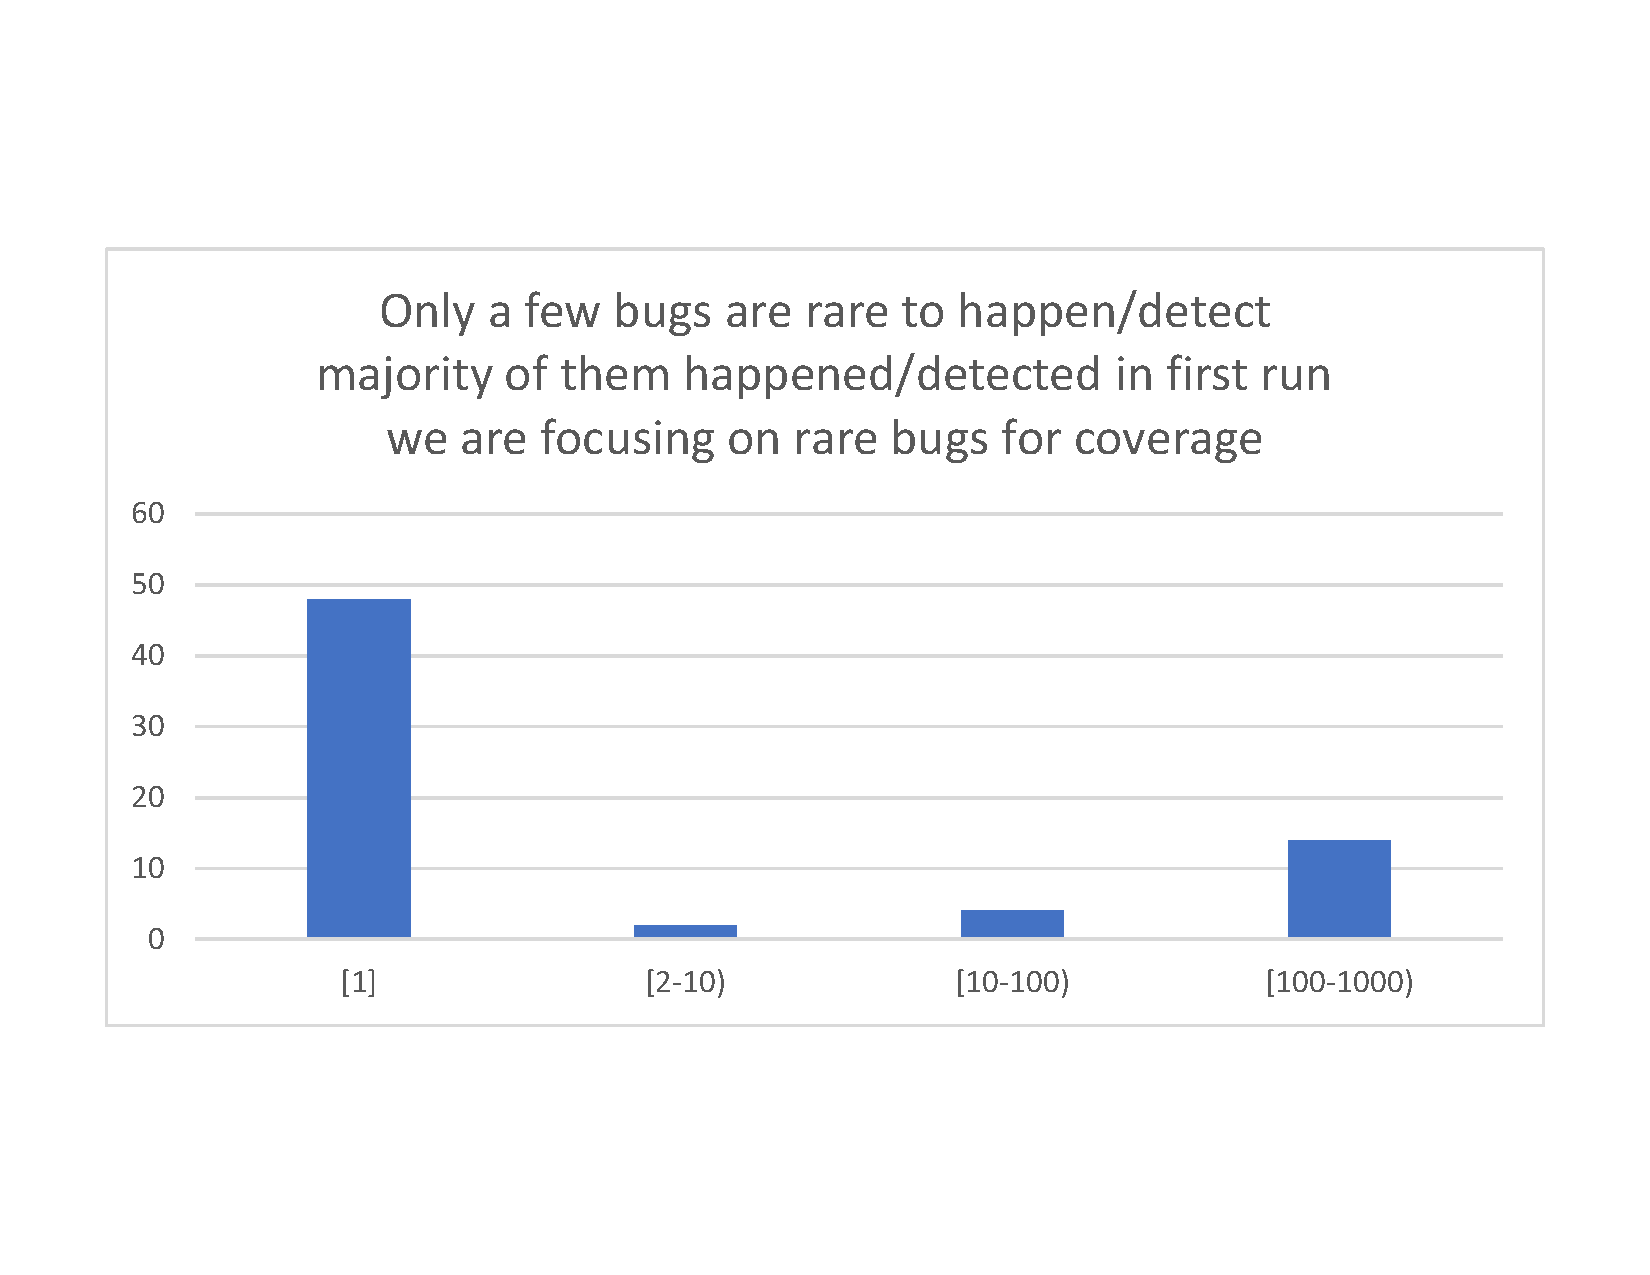
\includegraphics[width=.95\linewidth]{figs/coverage_motivation_tentative.pdf}
  \caption{focusing on rare bugs}
  \label{fig:rare_bugs}
\end{figure}



\subsection{Implementation}
Through a replay (\ie parsing the sequence) of ECT, a mapping between dynamic concurrent events and statically obtained CU points is emited by matching their respective call-stack and CU source location.
%
Through a BFS traversal of the goroutine tree, we add a \textit{coverage vector} to each goroutine node from the emitted mapping. Each element of the coverage vector is the respective covered value of requirement $R_i$ for the current goroutine node.
%
During executions of tests $t \in \mathcal{T}$, we maintain and update a global goroutine tree after each $t$.
%
It is crucial to maintain a global goroutine tree to measure the progress of coverage percentage over tests in $\mathcal{T}$.
%
Two goroutines $G_m$ and $G_n$ in the tests $t_i$ and $t_j$ are \textit{equivalent} (\ie falls into identical node in the global goroutine tree) if their parents are equivalent and their creation source location (CU of kind \texttt{go}) are identical:
\begin{equation}
  G_m \equiv G_n   \text{if}
  \begin{cases}
    \text{parent}(G_m) \equiv \text{parent}(G_n)  \wedge \\
    \text{CU(}G_m\text{).file} = \text{CU(}G_n\text{).file}  \wedge\\
    \text{CU(}G_m\text{).line} = \text{CU(}G_n\text{).line} \\
  \end{cases}
\end{equation}





\subsection{Evaluation}
We picked two representative bug kernels \texttt{etcd7443} and \texttt{kubernetes11298} to evaluate the coverage idea on them as they
%
They both have extensive use of channels, mutexes, conditional variables, nested selects within nested for loops and the buggy interleaving is proved to be rare to happen.
%
figures \ref{etcd_coverage} and \ref{fig:kubernetes_coverage} show the gradual increase in coverage percentage during execution runs for different values of D.
%
Recall that D is the bound on the number of yields that we inject to the native execution of a given program to perturb the scheduler around concurrency usages.
%
These figures show that
%

\begin{figure}
\centering
  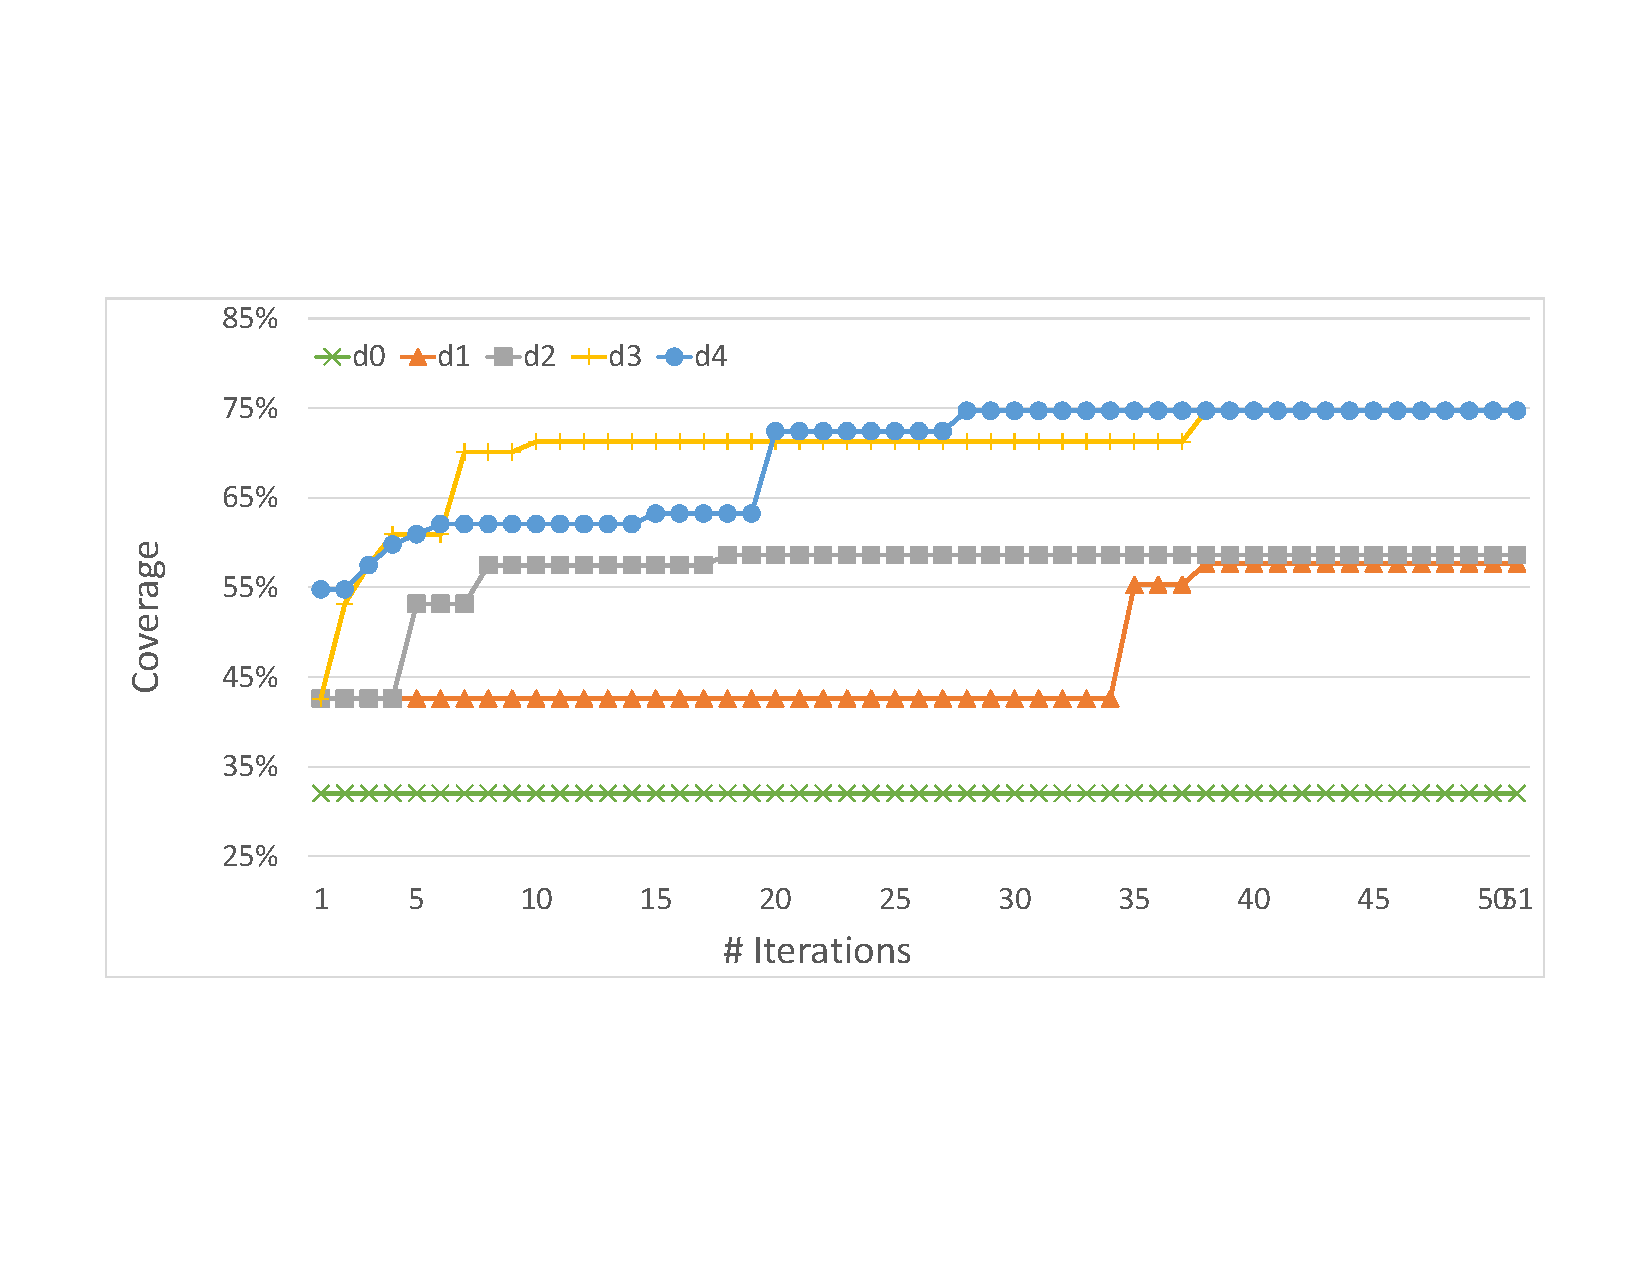
\includegraphics[width=.95\linewidth]{figs/coverage_etcd7443.pdf}
  \caption{etcd7442 coverage}
  \label{fig:etcd_coverage}
\end{figure}


\begin{figure}
\centering
  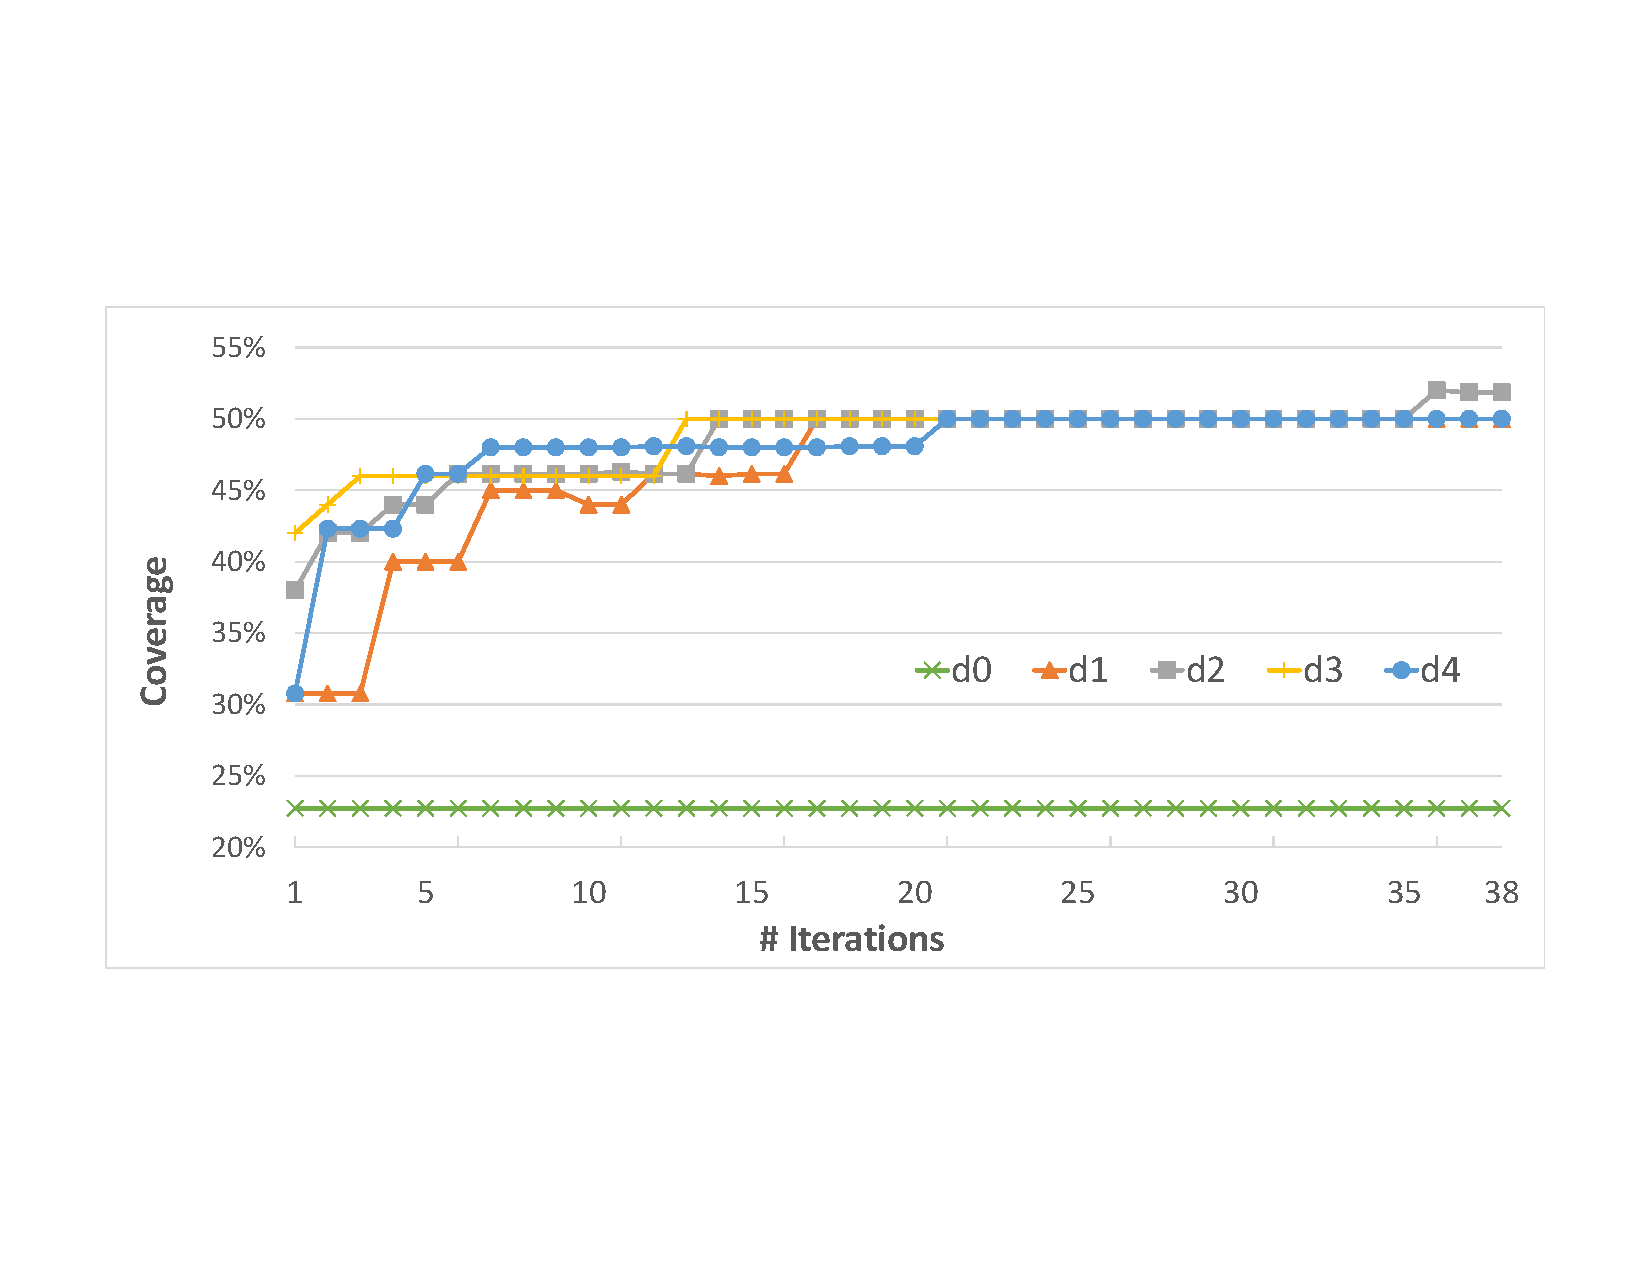
\includegraphics[width=.95\linewidth]{figs/coverage_kubernetes11298.pdf}
  \caption{kuberenetes11298 coverage}
  \label{fig:kubernetes_coverage}
\end{figure}
